\documentclass[11pt,a4paper]{article}

\usepackage[utf8]{inputenc}
\usepackage[margin=2.5cm]{geometry}
\usepackage{amsmath,amssymb}
\usepackage{graphicx}
\usepackage{booktabs}
\usepackage{float}
\usepackage{caption}
\usepackage{enumitem}
\usepackage{microtype}
\usepackage[hidelinks]{hyperref}

% Figures are generated by ponax_audit_forecasting.ipynb in the results/ folder at the root of the repository
\graphicspath{{../results/}}

\setlength{\parskip}{0.45em}
\setlength{\parindent}{0pt}
\setlist{itemsep=0.15em, topsep=0.3em}

\title{PONAX Bond Fund:\\ Factor Audit and Time-Series Forecasting}
\author{Justin Target, Jean-Athanas Iskander, Louise Mebarki,\\
Grâce Rabesandratana, Laurélie Sellahennedi, Anaïs Friedrich\\[0.6em]
\small ESILV --- Applied Financial Econometrics, Group 2\\[0.6em]
\footnotesize Original report written by Group 2 and submitted in French in October 2026.\\
\footnotesize This version was revised and translated by Justin Target for this repository.}
\date{}

\begin{document}

\maketitle

% =====================================================================
\section*{Summary}
\addcontentsline{toc}{section}{Summary}
% =====================================================================

This report studies PONAX (PIMCO Income A), a multi-sector bond fund that can invest up to half of its assets in high yield, over 119 months from February 2015 to December 2024. It answers two questions.

\textbf{1. Does the fund generate a significant Jensen's alpha once its exposures to market, interest rate and credit risk are taken into account?} We compare three factor models estimated by OLS: the Fama--French 3-factor model, a bond model that replaces SMB and HML with a term factor (TERM) and a default factor (DEF), and a combined model. The bond model is retained: it raises the adjusted $R^2$ from 0.518 to 0.669 and has the lowest BIC, while SMB and HML add nothing significant to it. The fund is significantly exposed to the equity market and to changes in term and credit spreads, but its alpha ($-0.84\%$ per year) is not significantly different from zero, including with heteroskedasticity-robust standard errors.

\textbf{2. Can the fund's past returns forecast its excess return better than the historical mean?} The residuals of the bond model are autocorrelated (Ljung--Box test at 12 lags), which suggests a time structure left unexplained. However, AIC and BIC both select an ARMA$(0,0)$ model for the excess return, i.e.\ a constant mean. On the twelve months of 2024, held out of the estimation, its forecast errors are identical to those of the historical mean.

\begin{table}[H]
\centering
\caption{Key results}
\footnotesize
\setlength{\tabcolsep}{4pt}
\begin{tabular}{lll}
\toprule
Question & Result & Evidence \\
\midrule
Best factor model & Bond model (Mkt-RF, TERM, DEF) & Adj.\ $R^2$ 0.669, lowest BIC ($-783.7$) \\
Value of TERM and DEF & Significant & Joint F-test, $p \simeq 4.8 \times 10^{-11}$ \\
Value of SMB and HML & Not significant & Joint F-test, $p \simeq 0.081$ \\
Jensen's alpha & $-0.0007$ per month, not significant & $p = 0.413$ (OLS), $0.468$ (White HC1) \\
Residual autocorrelation & Present & Ljung--Box (12 lags), $p = 0.001$ \\
Best ARMA model & ARMA$(0,0)$, i.e.\ a constant & Lowest AIC and BIC over $p, q \le 3$ \\
2024 backtest & No gain over the historical mean & RMSE 0.0128 for both \\
\bottomrule
\end{tabular}
\end{table}

\textbf{Conclusion.} PONAX's performance is explained by the risks it takes rather than by abnormal returns, and its past returns contain no information that an ARMA model can use to forecast it.

\newpage
\setcounter{tocdepth}{1}
\tableofcontents
\bigskip

% =====================================================================
\section{Introduction}
% =====================================================================

\subsection{Economic question}

A quantitative audit of an actively managed fund asks whether its past performance reflects the manager's skill or simply its exposure to systematic risk factors that any investor can access. For a bond fund, returns depend largely on changes in interest rates, which affect bond prices through duration\footnote{See Section~4.10 of John Hull, \emph{Options, Futures, and Other Derivatives}, 11th edition.}, and on the compensation investors require for default risk and for changes in credit risk premia.

Our central question is therefore:
\begin{center}
\emph{Does PONAX's Jensen's alpha remain significant once its main exposures to market, interest rate and credit risk are taken into account?}
\end{center}

The answer matters for asset managers, wealth managers and private bankers: it tells them whether the fund's performance justifies its management fees given the risks actually taken.

\subsection{The fund}

PONAX (PIMCO Income A) invests at least 65\% of its assets in a multi-sector portfolio of fixed income instruments with varied maturities, issuers and credit quality. It can invest up to 50\% in high yield bonds and can also use derivatives such as options and swaps. Launched in 2007, it manages about 15 billion dollars.

\subsection{Approach}

Part~I explains the fund's excess returns with factor models. Because PONAX is a bond fund, the equity factors SMB and HML are unlikely to be sufficient, so we compare three models estimated on the same sample with the same dependent variable: the Fama--French 3-factor model as the reference, a bond model with term and default factors, and a combined model. We then check the assumptions of the retained model with a full set of diagnostics.

Part~II starts from what the retained model does not explain. It tests whether its residuals still contain a time structure, then asks whether the fund's own past returns can forecast its excess return better than the historical mean, using an ARMA model evaluated out of sample on 2024.

% =====================================================================
\part{Factor Audit}
% =====================================================================

\section{Data}

\subsection{Sources}

\begin{table}[H]
\centering
\caption{Data sources (monthly, January 2015 to December 2024)}
\footnotesize
\begin{tabular}{lll}
\toprule
Series & Source & Identifier \\
\midrule
PONAX adjusted closing prices & Yahoo Finance (\texttt{yfinance}) & PONAX \\
Mkt-RF, SMB, HML and risk-free rate RF & Kenneth French Data Library & F-F\_Research\_Data\_Factors \\
Moody's Baa corporate bond yield & FRED & DBAA \\
10-year US Treasury yield & FRED & DGS10 \\
3-month US Treasury bill rate & FRED & DTB3 \\
\bottomrule
\end{tabular}
\end{table}

Prices are adjusted for dividends and corporate actions, so that distributions do not create artificial jumps in returns. The FRED series are monthly averages.

\subsection{Variables}

The monthly return of PONAX is the log return of its adjusted price, and its excess return is $R^e_{\text{PONAX},t} = R_{\text{PONAX},t} - R_{f,t}$, with $R_f$ from the Kenneth French Data Library.

The two bond factors are built from changes in rates:
\[
\text{TERM}_t = \Delta \text{DGS10}_t - \Delta \text{DTB3}_t,
\qquad
\text{DEF}_t = \Delta \text{DBAA}_t - \Delta \text{DGS10}_t,
\]
where $\Delta X_t = X_t - X_{t-1}$.
TERM measures the change in the slope of the Treasury curve and captures duration risk. DEF measures the change in the spread between Baa corporate bonds and Treasuries and captures credit risk. Since these series are rates rather than prices, we use simple differences rather than log changes. All series are converted from percent to decimals.

\subsection{Sample and preprocessing}

January 2015 is dropped because returns and rate changes require the previous month, which leaves 119 monthly observations. Zero values of RF are genuine observations and are kept.

One caveat applies throughout the study: the rates are monthly averages, so their changes run from mid-month to mid-month, while fund returns run from month end to month end. This slight calendar mismatch should be kept in mind when interpreting the factor loadings.

We flag outliers with the IQR rule (below $Q_1 - 1.5\,\text{IQR}$ or above $Q_3 + 1.5\,\text{IQR}$) and examine them before any removal.

\begin{table}[H]
\centering
\caption{Outliers detected with the IQR rule}
\footnotesize
\setlength{\tabcolsep}{4pt}
\begin{tabular}{lrrrrrp{4.4cm}}
\toprule
Variable & $Q_1$ & $Q_3$ & Lower bound & Upper bound & N & Dates \\
\midrule
$R_i - R_f$ & $-0.0043$ & $0.0083$ & $-0.0233$ & $0.0272$ & 10 & 2020-03, 2022-02, 2022-04, 2022-06, 2022-07, 2022-09, 2022-11, 2023-01, 2023-02, 2023-11 \\
Mkt-RF & $-0.0155$ & $0.0344$ & $-0.0903$ & $0.1091$ & 6 & 2018-12, 2020-03, 2020-04, 2020-11, 2022-04, 2022-09 \\
SMB & $-0.0232$ & $0.0154$ & $-0.0812$ & $0.0734$ & 0 & -- \\
HML & $-0.0215$ & $0.0170$ & $-0.0792$ & $0.0748$ & 6 & 2016-11, 2020-03, 2022-01, 2022-05, 2022-10, 2023-03 \\
TERM & $-0.0012$ & $0.0011$ & $-0.0047$ & $0.0046$ & 4 & 2020-03, 2022-07, 2022-11, 2024-10 \\
DEF & $-0.0010$ & $0.0005$ & $-0.0031$ & $0.0027$ & 4 & 2016-03, 2020-03, 2020-06, 2022-05 \\
\bottomrule
\end{tabular}
\end{table}

The rule flags 30 values. They cluster around two real market events: March 2020, which appears for five variables, and the 2022--2023 rate hikes. Since they reflect how the fund behaves under stress rather than data errors, all of them are kept.

\section{Exploratory analysis}

\subsection{Distributions}

\begin{figure}[H]
\centering
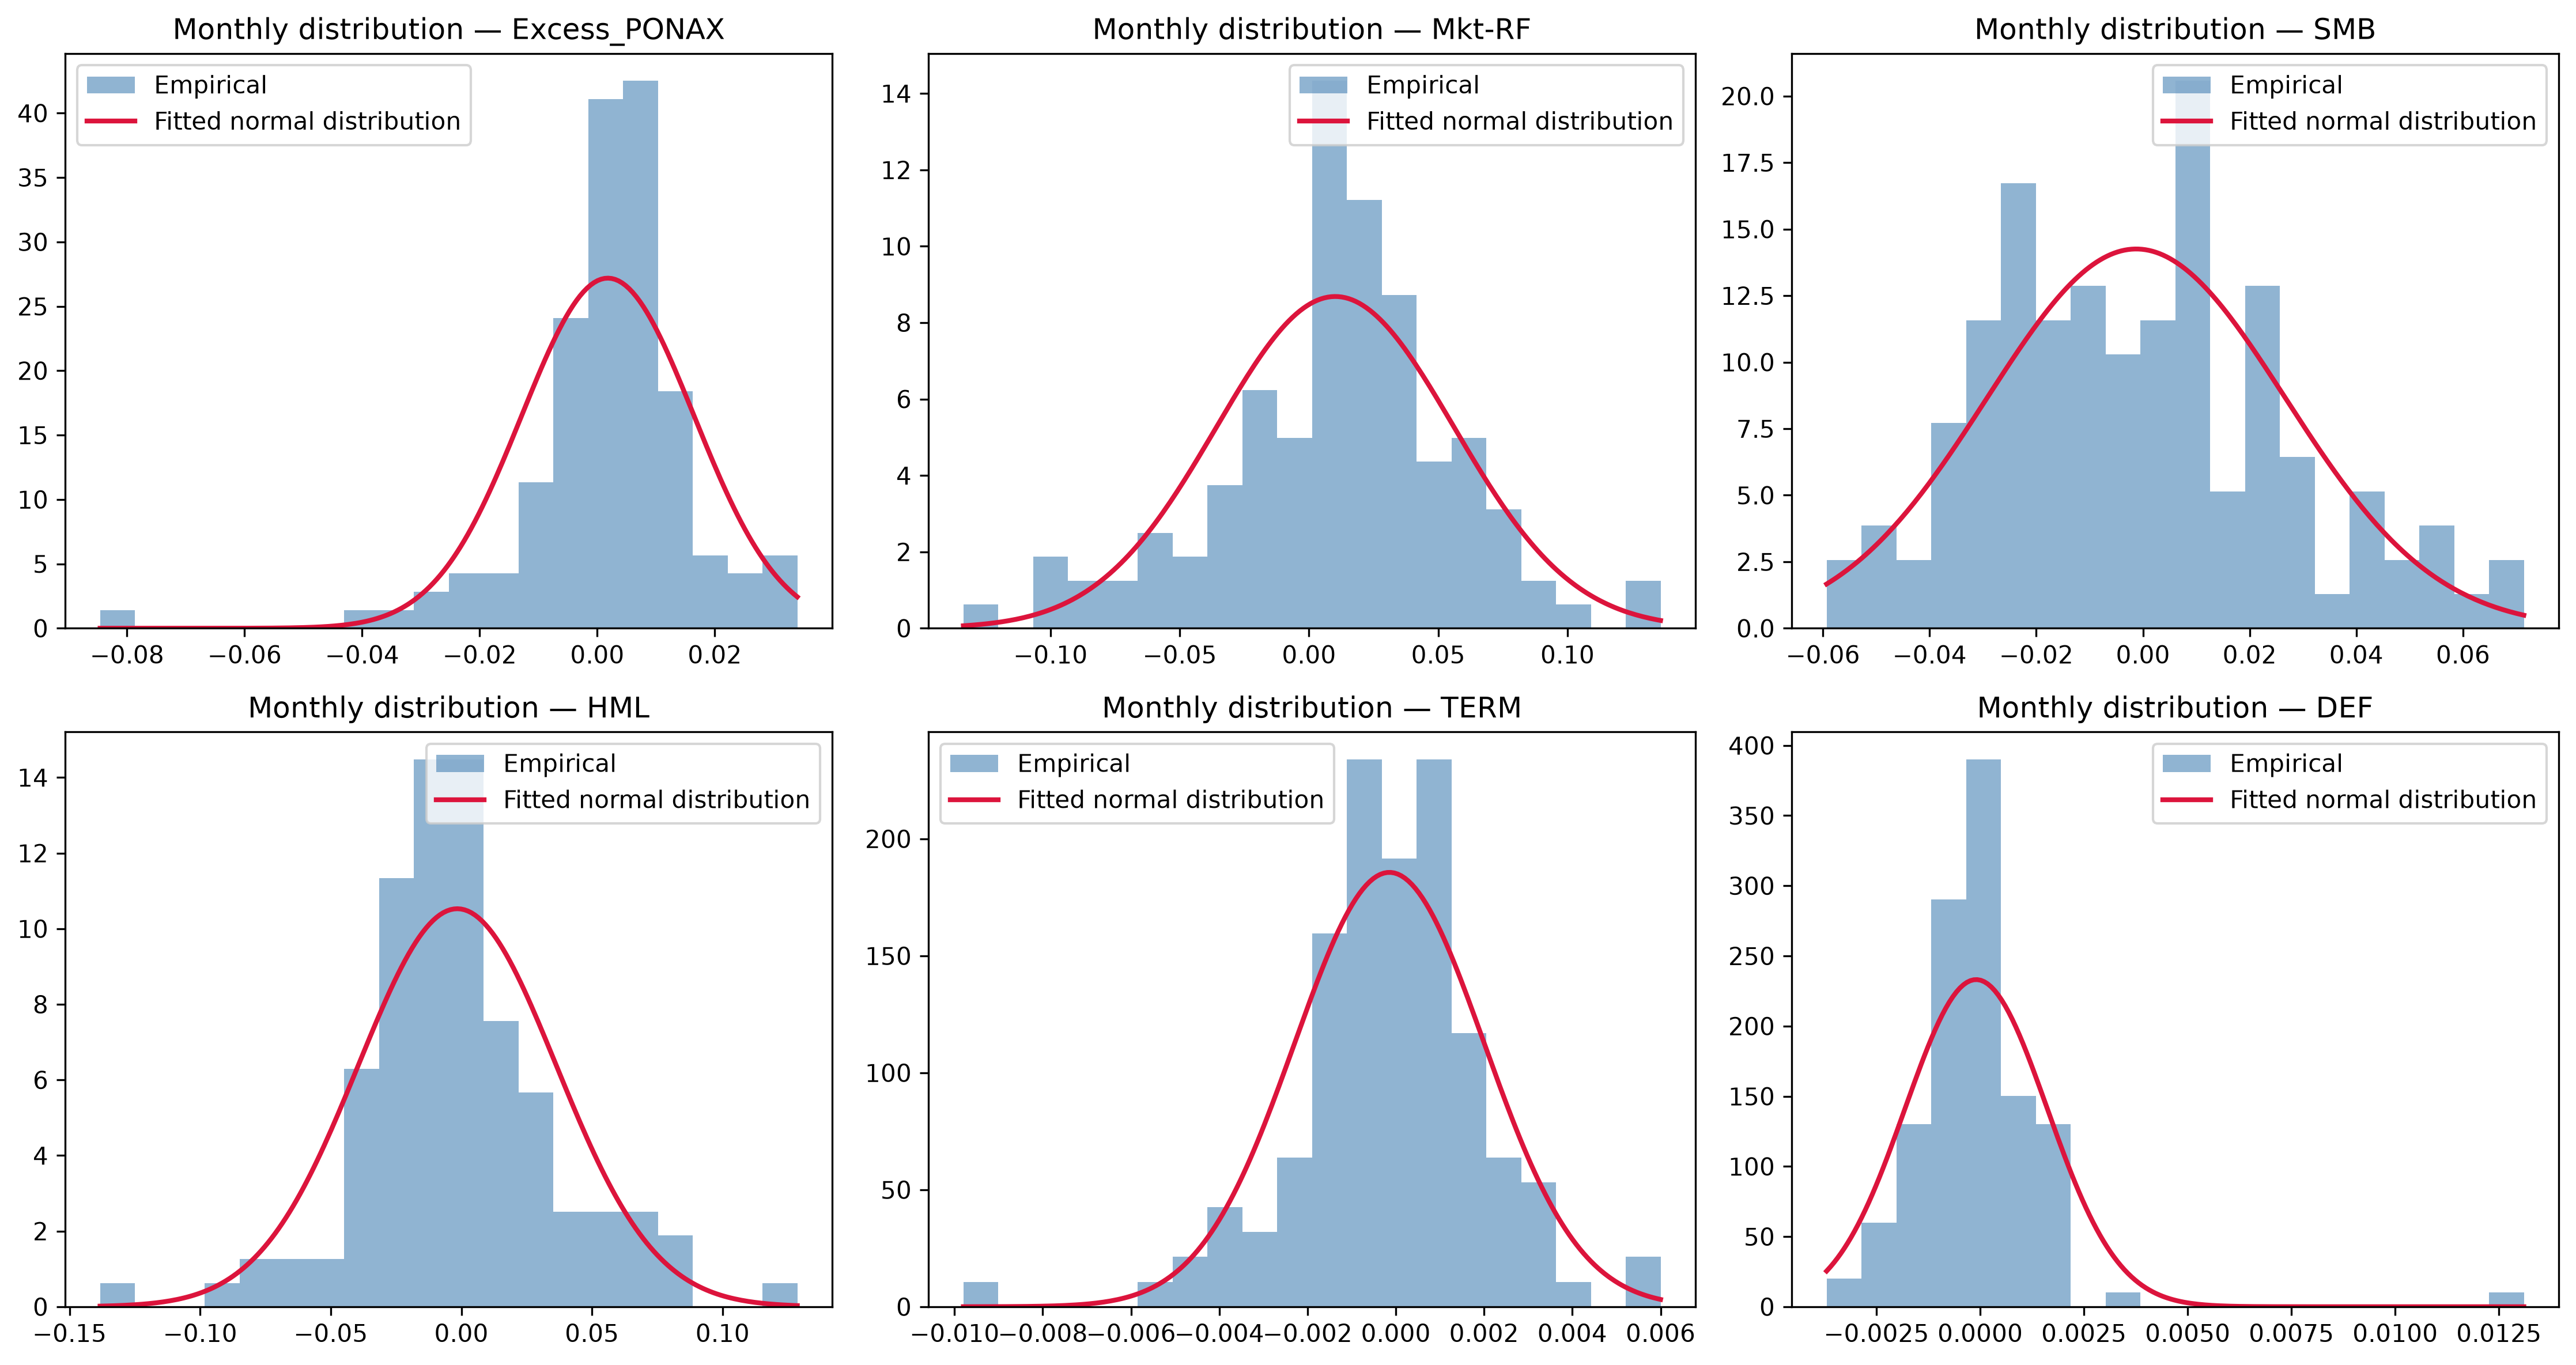
\includegraphics[width=\textwidth]{histograms_normality.png}
\caption{Distributions of the regression variables and fitted normal densities}
\label{fig:hist}
\end{figure}

\begin{table}[H]
\centering
\caption{Descriptive statistics and Jarque--Bera normality test}
\small
\begin{tabular}{lrrrrrr}
\toprule
Variable & Mean & Std.\ dev. & Skewness & Kurtosis & JB & JB p-value \\
\midrule
$R_i - R_f$ & 0.0018 & 0.0147 & $-1.94$ & 12.96 & 520.18 & 0.0000 \\
Mkt-RF & 0.0102 & 0.0459 & $-0.36$ & 3.74 & 4.63 & 0.0988 \\
SMB & $-0.0013$ & 0.0280 & 0.41 & 2.80 & 3.49 & 0.1747 \\
HML & $-0.0016$ & 0.0379 & 0.22 & 4.92 & 16.90 & 0.0002 \\
TERM & $-0.0001$ & 0.0021 & $-0.55$ & 6.30 & 53.90 & 0.0000 \\
DEF & $-0.0001$ & 0.0017 & 3.82 & 32.28 & 4174.37 & 0.0000 \\
\bottomrule
\end{tabular}

\smallskip
\footnotesize Kurtosis is the raw kurtosis (3 for a normal distribution).
\label{tab:desc}
\end{table}

PONAX's excess return has low volatility: most months are more concentrated around the mean than a normal distribution would predict. Its distribution is nonetheless far from normal, with a strong negative skew ($-1.94$) and fat tails (kurtosis of 13.0): extreme months are more frequent than under normality, and they are more often losses than gains. The Jarque--Bera test does not reject normality for Mkt-RF and SMB, but rejects it at the 5\% level for HML, TERM, DEF and the fund's excess return.

Non-normal variables do not invalidate OLS estimates: what matters for inference is the distribution of the residuals, tested in Section~\ref{sec:diag}.

\subsection{Correlations}

\begin{table}[H]
\centering
\caption{Correlation matrix of the factors}
\small
\begin{tabular}{lrrrrr}
\toprule
 & Mkt-RF & SMB & HML & TERM & DEF \\
\midrule
Mkt-RF & 1.000 & 0.297 & 0.026 & $-0.145$ & $-0.310$ \\
SMB & 0.297 & 1.000 & 0.113 & $-0.074$ & $-0.218$ \\
HML & 0.026 & 0.113 & 1.000 & 0.156 & $-0.286$ \\
TERM & $-0.145$ & $-0.074$ & 0.156 & 1.000 & $-0.022$ \\
DEF & $-0.310$ & $-0.218$ & $-0.286$ & $-0.022$ & 1.000 \\
\bottomrule
\end{tabular}
\end{table}

\begin{figure}[H]
\centering
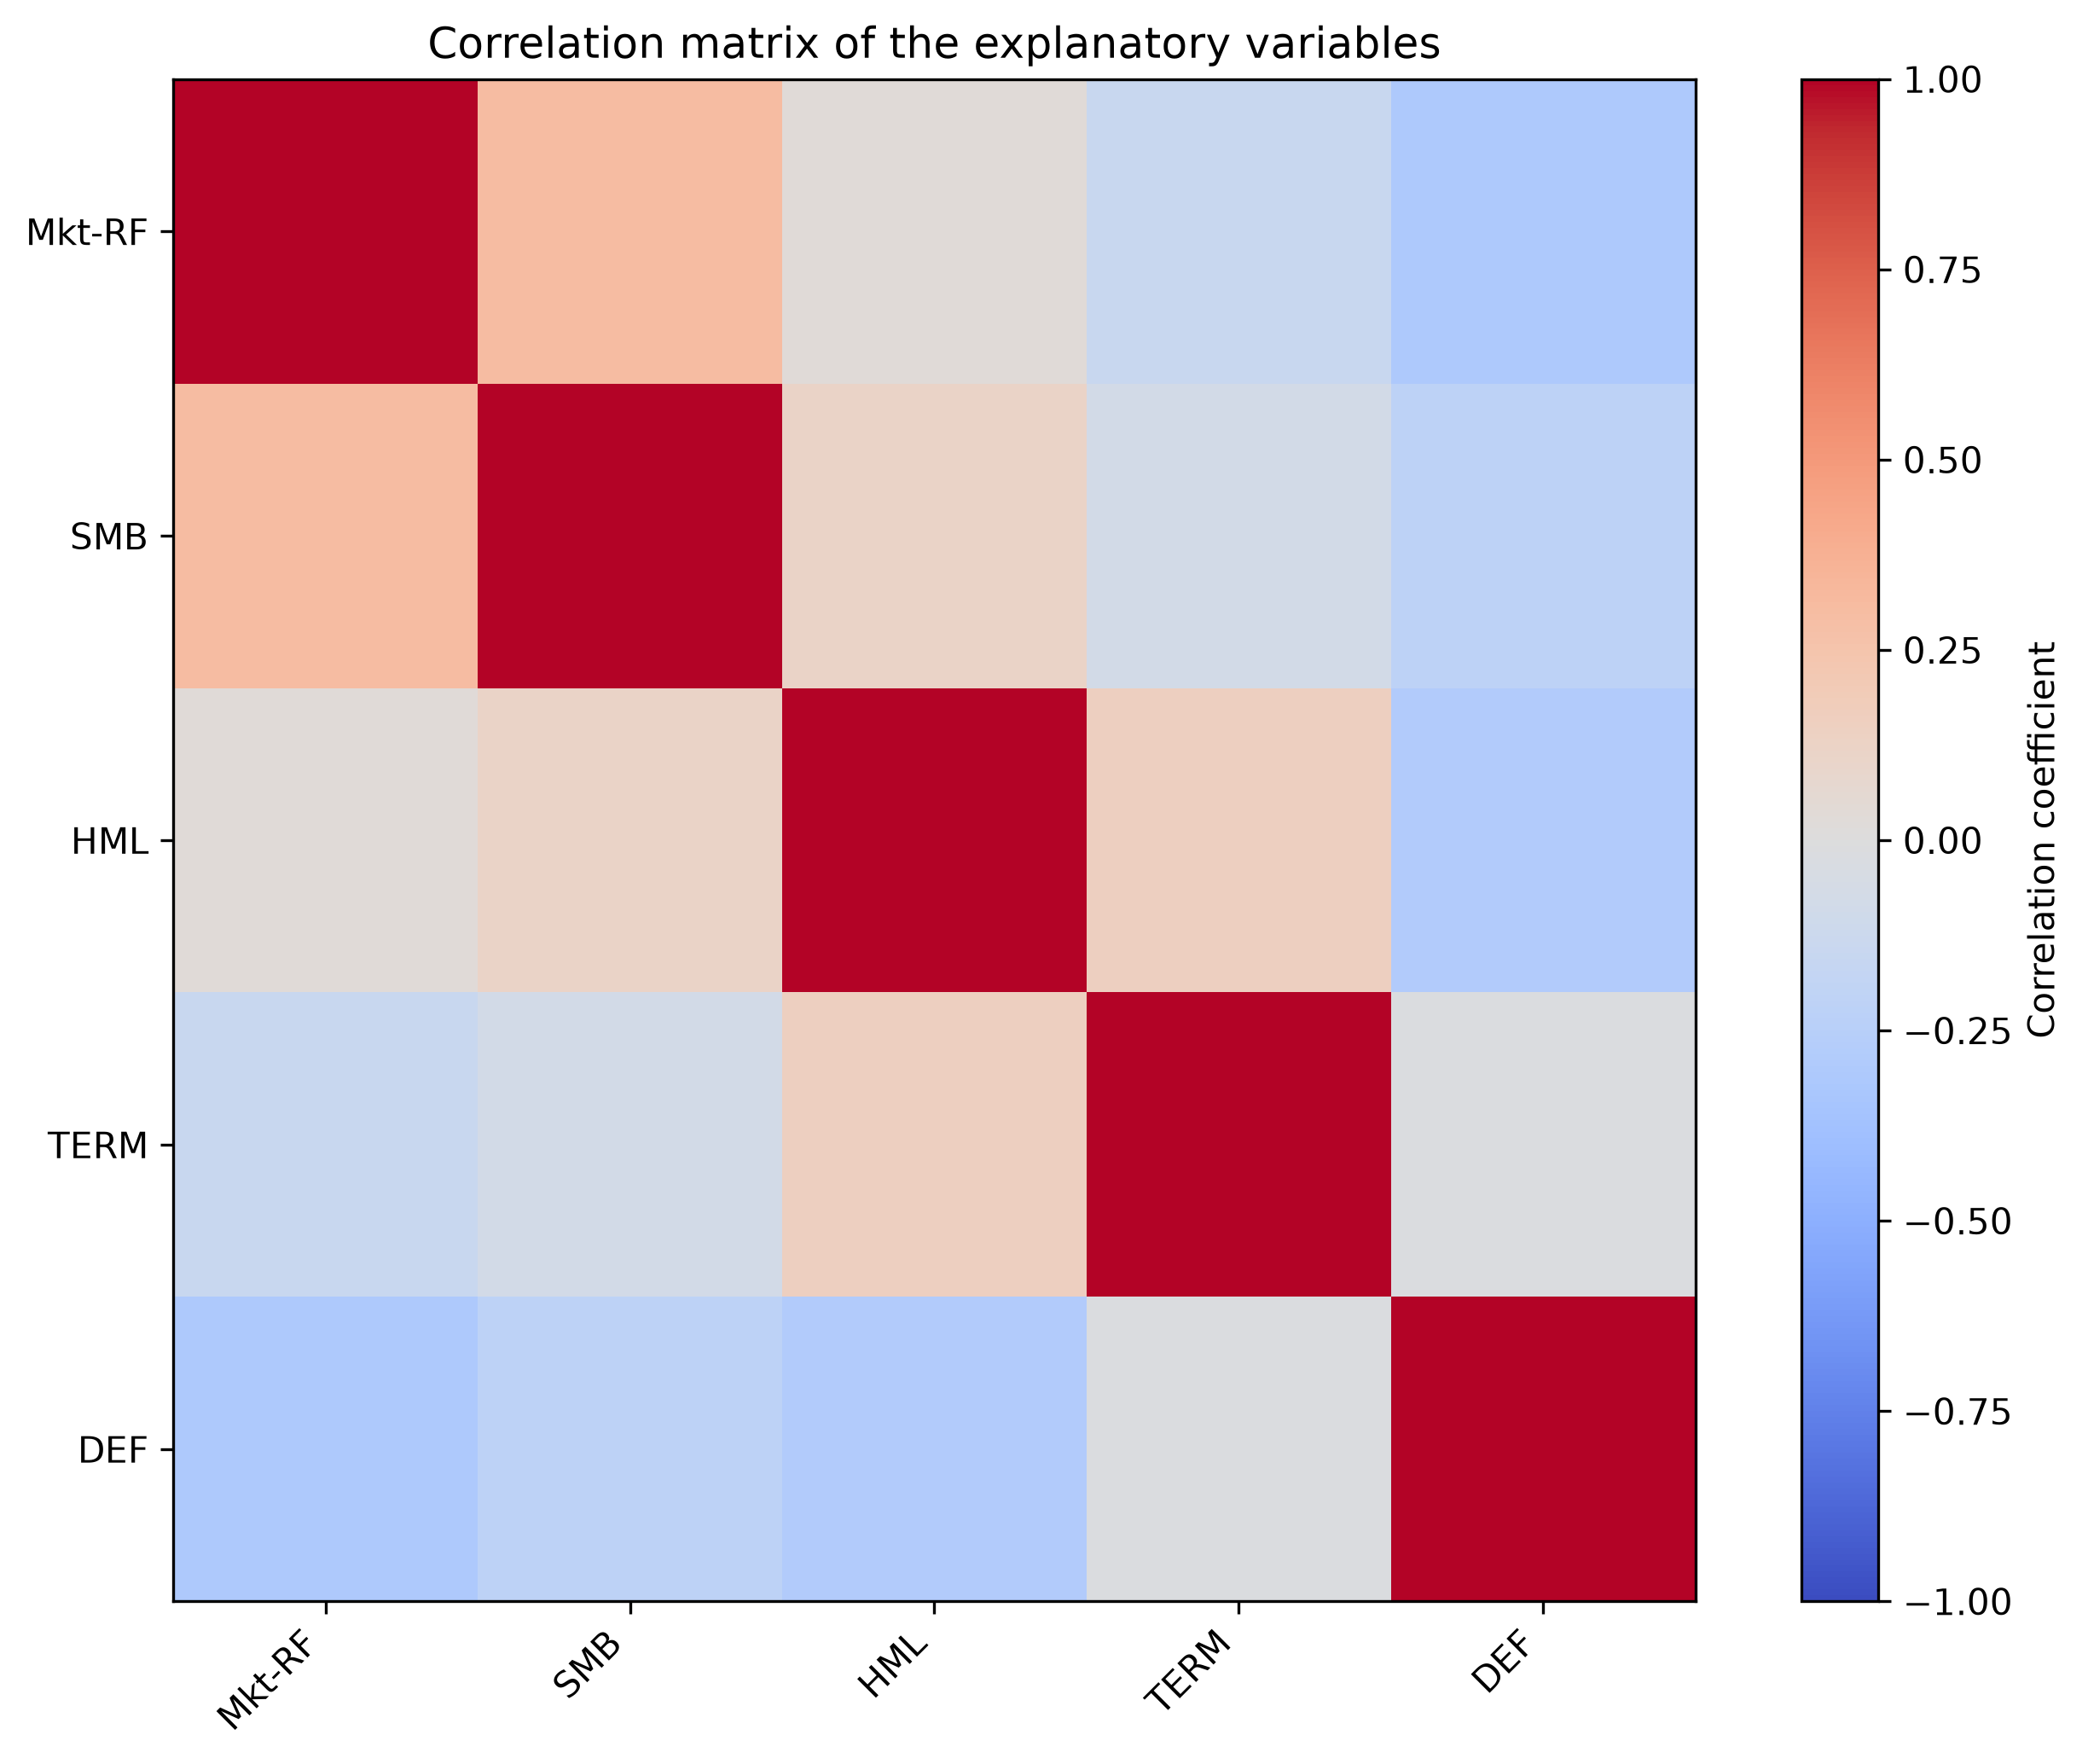
\includegraphics[width=0.55\textwidth]{correlation_heatmap.png}
\caption{Correlation heatmap of the factors}
\end{figure}

Correlations between factors are weak: the largest in absolute value is $-0.310$, between Mkt-RF and DEF. Multicollinearity is therefore unlikely, which the VIF confirms in Section~\ref{sec:diag}.

\section{Models}

\subsection{Specifications}

The reference model is the Fama--French 3-factor model:
\begin{equation}
R^e_{\text{PONAX},t} = \alpha + \beta_1 (R_{m,t} - R_{f,t}) + \beta_2\,\text{SMB}_t + \beta_3\,\text{HML}_t + \varepsilon_t,
\end{equation}
where $\alpha$ is Jensen's alpha, the average excess return not explained by the factors, and $\beta_1$, $\beta_2$, $\beta_3$ measure the fund's exposure to the equity market, to small caps relative to large caps, and to value relative to growth stocks.

SMB and HML are built from characteristics of listed companies, so nothing guarantees that they explain the returns of a bond fund. In their 1993 paper, Fama and French also propose two bond factors, TERM and DEF. Given PONAX's investment universe, we replace SMB and HML with these factors in the bond model:
\begin{equation}
R^e_{\text{PONAX},t} = \alpha + \beta_1 (R_{m,t} - R_{f,t}) + \gamma_1\,\text{TERM}_t + \gamma_2\,\text{DEF}_t + \varepsilon_t.
\end{equation}
The combined model includes all five factors and nests the two previous models:
\begin{equation}
R^e_{\text{PONAX},t} = \alpha + \beta_1 (R_{m,t} - R_{f,t}) + \beta_2\,\text{SMB}_t + \beta_3\,\text{HML}_t + \gamma_1\,\text{TERM}_t + \gamma_2\,\text{DEF}_t + \varepsilon_t.
\end{equation}

\paragraph{Expected signs.} TERM and DEF are changes in rates, not bond returns, and bond prices fall when yields rise. For a fund with positive duration, we therefore expect $\gamma_1 < 0$. Likewise, a wider credit spread hurts a portfolio exposed to credit, so we expect $\gamma_2 < 0$.

\subsection{Estimation}

The three models are estimated by OLS with \texttt{statsmodels}, $\hat{\beta} = (X^\top X)^{-1} X^\top y$, with a constant to estimate the alpha. Inference relies on the usual assumptions: linearity, exogenous regressors, homoskedastic and uncorrelated errors, a full-rank design matrix and, for exact tests in a small sample, normal errors. Section~\ref{sec:diag} tests each of them.

\begin{table}[H]
\centering
\caption{OLS estimates (standard errors in parentheses)}
\small
\begin{tabular}{lrrr}
\toprule
 & Fama--French & Bond & Combined \\
\midrule
Constant ($\alpha$) & $-0.0003$ & $-0.0007$ & $-0.0006$ \\
 & (0.0010) & (0.0008) & (0.0008) \\
Mkt-RF & 0.2216 & 0.1853 & 0.1861 \\
 & (0.0214) & (0.0180) & (0.0183) \\
SMB & 0.0297 & -- & 0.0068 \\
 & (0.0353) & & (0.0290) \\
HML & 0.0499 & -- & 0.0489 \\
 & (0.0249) & & (0.0214) \\
TERM & -- & $-2.3309$ & $-2.4507$ \\
 & & (0.3663) & (0.3656) \\
DEF & -- & $-2.3291$ & $-1.9917$ \\
 & & (0.4787) & (0.4954) \\
\midrule
$R^2$ & 0.531 & 0.678 & 0.692 \\
Adjusted $R^2$ & 0.5183 & 0.6694 & 0.6788 \\
BIC & $-738.90$ & $-783.68$ & $-779.66$ \\
N & 119 & 119 & 119 \\
\bottomrule
\end{tabular}
\label{tab:ols}
\end{table}

\section{Results}

\subsection{Model selection}

Adding the bond factors strongly improves the reference model: the adjusted $R^2$ rises from 0.518 to 0.669 and the BIC falls from $-738.9$ to $-783.7$. The combined model fits slightly better still, with an adjusted $R^2$ of 0.679 and the lowest AIC ($-796.3$), but its BIC ($-779.7$) is worse than that of the bond model. Since the BIC penalizes additional parameters more heavily than the AIC, it favors the more parsimonious bond model.

Two Fisher tests on the nested models confirm this choice, using the unadjusted $R^2$ of Table~\ref{tab:ols}:
\begin{itemize}
\item TERM and DEF add significant information to the Fama--French model ($H_0: \gamma_1 = \gamma_2 = 0$):
\[
F = \frac{(0.692 - 0.531)/2}{(1 - 0.692)/113} \simeq 29.53, \qquad p \simeq 4.8 \times 10^{-11}.
\]
\item SMB and HML do not add significant information to the bond model at the 5\% level ($H_0: \beta_2 = \beta_3 = 0$):
\[
F = \frac{(0.692 - 0.678)/2}{(1 - 0.692)/113} \simeq 2.57, \qquad p \simeq 0.081.
\]
\end{itemize}

The bond model is therefore retained for the rest of the study.

\subsection{Jensen's alpha}

A non-zero estimated alpha can simply reflect sampling noise over 119 months, so we test $H_0: \alpha = 0$ against $H_1: \alpha \neq 0$ with a Student test with 115 degrees of freedom.

The estimated alpha is $-0.0007$ per month, about $-0.84\%$ per year (12 times the monthly value, since returns are log returns). Its t-statistic is $-0.822$ and its p-value 0.413, so $H_0$ is not rejected at the 5\% level. The result holds with White robust standard errors ($p = 0.468$, Section~\ref{sec:diag}).

\textbf{Answer to the first question:} once exposures to the equity market, interest rate risk and credit risk are controlled for, PONAX's alpha is not significantly different from zero. This does not prove that the alpha is zero: with 119 months, a small outperformance would be hard to detect.

\subsection{Factor exposures}

All three exposures are significant at the 1\% level and have the expected signs.
\begin{itemize}
\item \textbf{Equity market} ($\beta_1 = 0.185$): when the market excess return rises by 1 point, PONAX's excess return rises by 0.19 point on average. This low sensitivity is consistent with a bond fund, but shows that PONAX remains somewhat exposed to equities.
\item \textbf{Interest rates} ($\gamma_1 = -2.33$): a 10 basis point increase in TERM, i.e.\ a steepening of the Treasury curve, lowers the monthly return by about 0.23 point.
\item \textbf{Credit} ($\gamma_2 = -2.33$): a 10 basis point widening of the credit spread lowers the monthly return by about 0.23 point, consistent with the fund's ability to invest up to 50\% in high yield.
\end{itemize}
Since the factors are built from monthly average rates, these magnitudes should be read as approximate.

\section{Diagnostics of the bond model}
\label{sec:diag}

\begin{table}[H]
\centering
\caption{Summary of the diagnostics}
\footnotesize
\setlength{\tabcolsep}{4pt}
\begin{tabular}{lllp{4.3cm}}
\toprule
Assumption & Test & Result & Consequence \\
\midrule
Linearity & RESET & Rejected at 5\% ($p = 0.0176$) & Loadings read as average sensitivities \\
Homoskedasticity & Breusch--Pagan & Rejected ($p = 0.0001$) & White HC1 standard errors \\
Normal residuals & Jarque--Bera & Not rejected ($p = 0.116$) & Usual inference acceptable \\
Influential points & Cook's distance & 6 above $4/n$ & Kept; March 2020 dominant \\
Multicollinearity & VIF & All below 1.2 & No action needed \\
No autocorrelation & DW, Breusch--Godfrey & Not rejected ($p = 0.065$) & No correction needed \\
\bottomrule
\end{tabular}
\end{table}

\subsection{Linearity}

The RESET test adds the squared and cubed fitted values to the model and checks with a Fisher test whether they carry information. Its p-value is 0.0176: linearity is rejected at the 5\% level, but not at the 1\% level. The residuals show no clear curvature against the fitted values (Figure~\ref{fig:resfit}), apart from one isolated point with a very negative fitted value. A non-linear effect or an omitted factor cannot be ruled out, so the loadings should be read as average sensitivities over the period.

\begin{figure}[H]
\centering
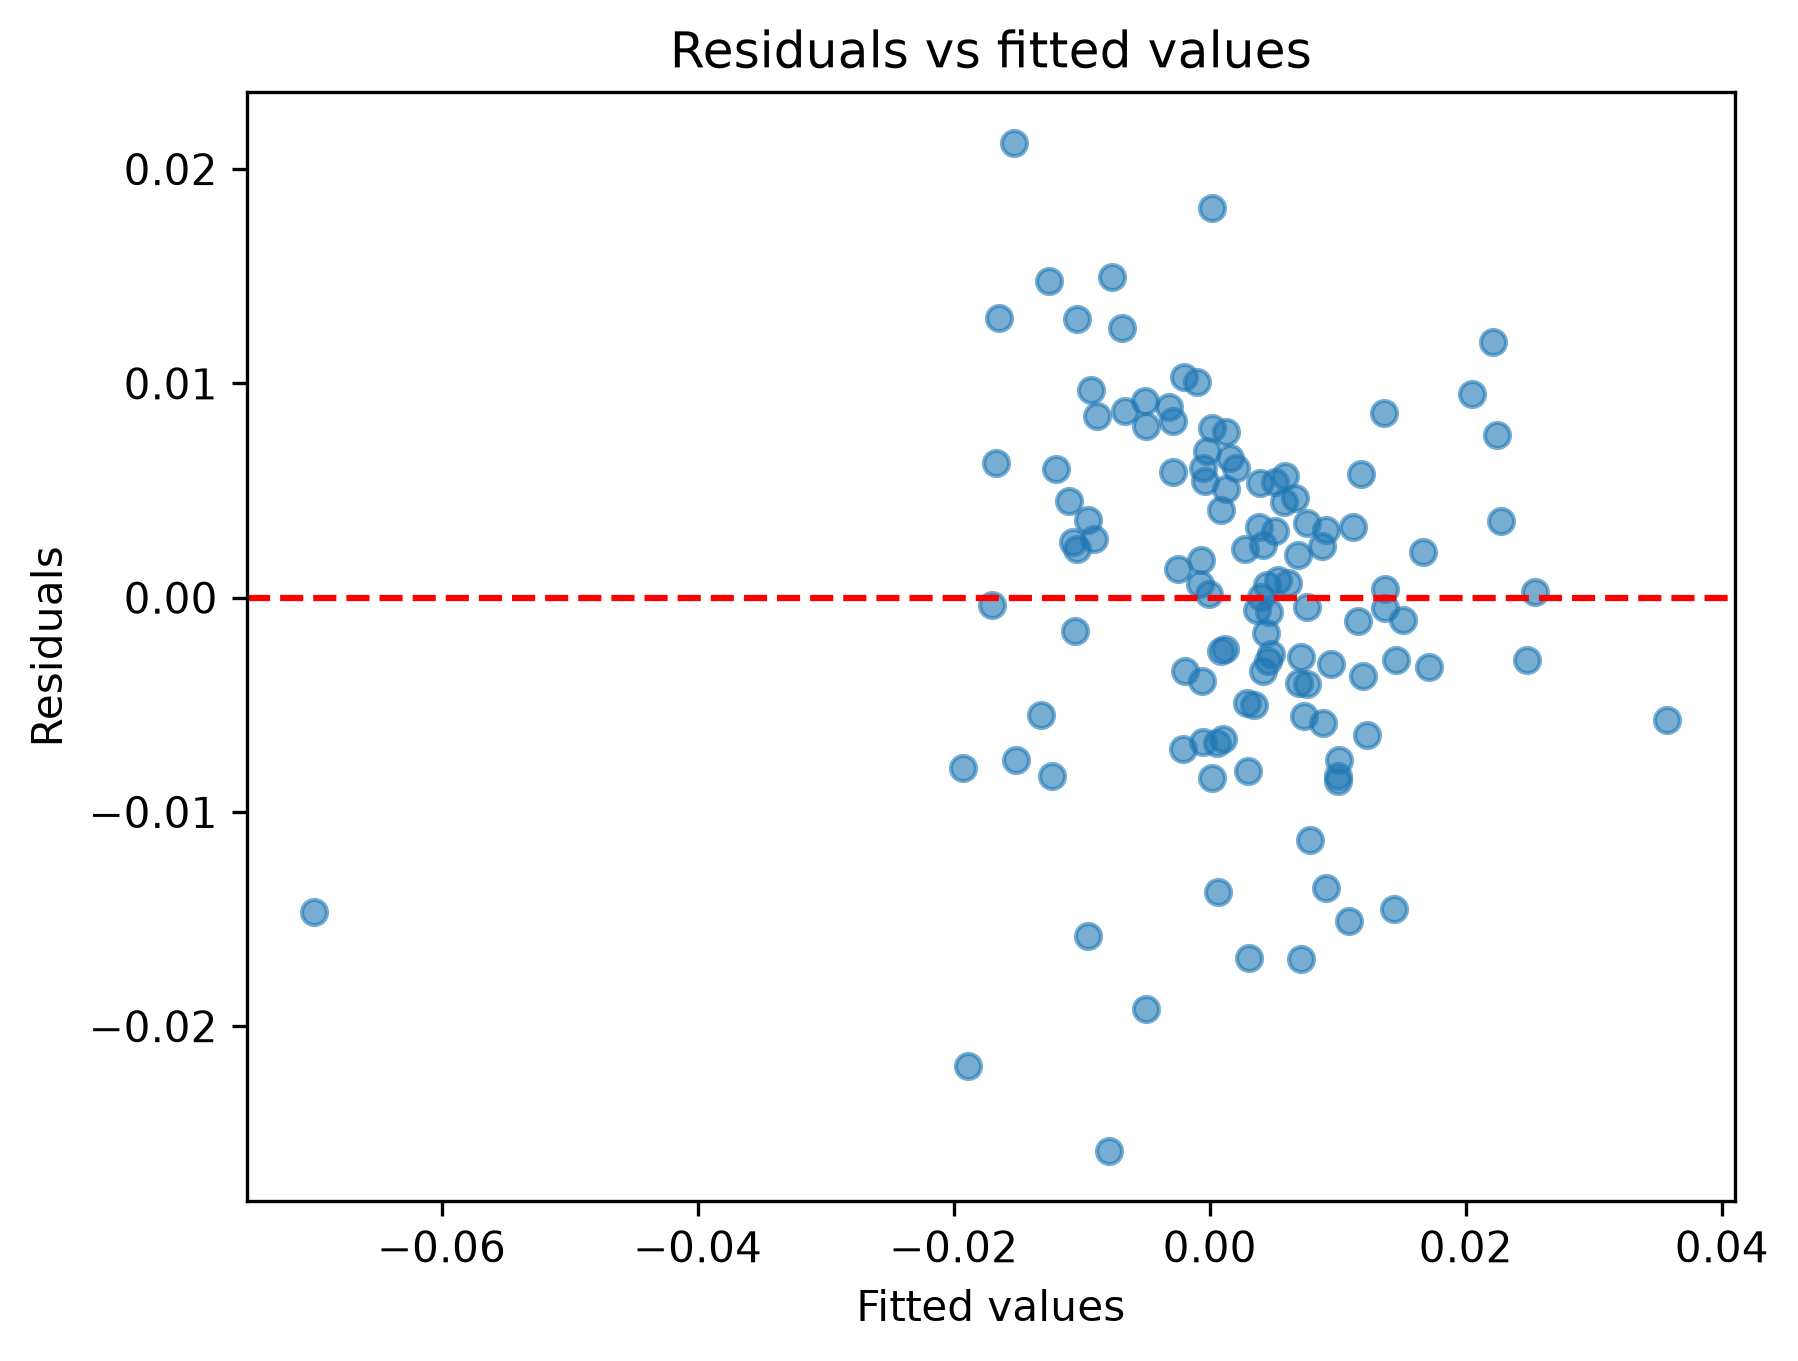
\includegraphics[width=0.55\textwidth]{residuals_vs_fitted.png}
\caption{Residuals of the bond model against fitted values}
\label{fig:resfit}
\end{figure}

\subsection{Homoskedasticity}

If the error variance is not constant, OLS estimates remain unbiased but the usual standard errors, t-statistics and p-values are no longer reliable. The Breusch--Pagan test rejects homoskedasticity ($p = 0.0001$), so we re-estimate the model with White robust standard errors (HC1). The coefficients are unchanged and only their standard errors increase. None of the conclusions change: the alpha remains non-significant and the three factors remain significant at the 1\% level.

\begin{table}[H]
\centering
\caption{Classic and White (HC1) standard errors of the bond model}
\small
\begin{tabular}{lrrrr}
\toprule
 & p-value (OLS) & p-value (HC1) & Std.\ error (OLS) & Std.\ error (HC1) \\
\midrule
$\alpha$ & 0.413 & 0.468 & 0.0008 & 0.0009 \\
Mkt-RF & $< 0.001$ & $< 0.001$ & 0.018 & 0.026 \\
TERM & $< 0.001$ & $< 0.001$ & 0.366 & 0.431 \\
DEF & $< 0.001$ & $< 0.001$ & 0.479 & 0.691 \\
\bottomrule
\end{tabular}
\end{table}

\subsection{Normality of the residuals}

Normal errors are needed for the Student and Fisher tests to be exact in a small sample. The Jarque--Bera statistic of the residuals is 4.315, with a p-value of 0.116, so normality is not rejected. The Q-Q plot (Figure~\ref{fig:qq}) agrees: the points follow the line except in the left tail, where a few very negative months are more extreme than a normal distribution would predict.

\begin{figure}[H]
\centering
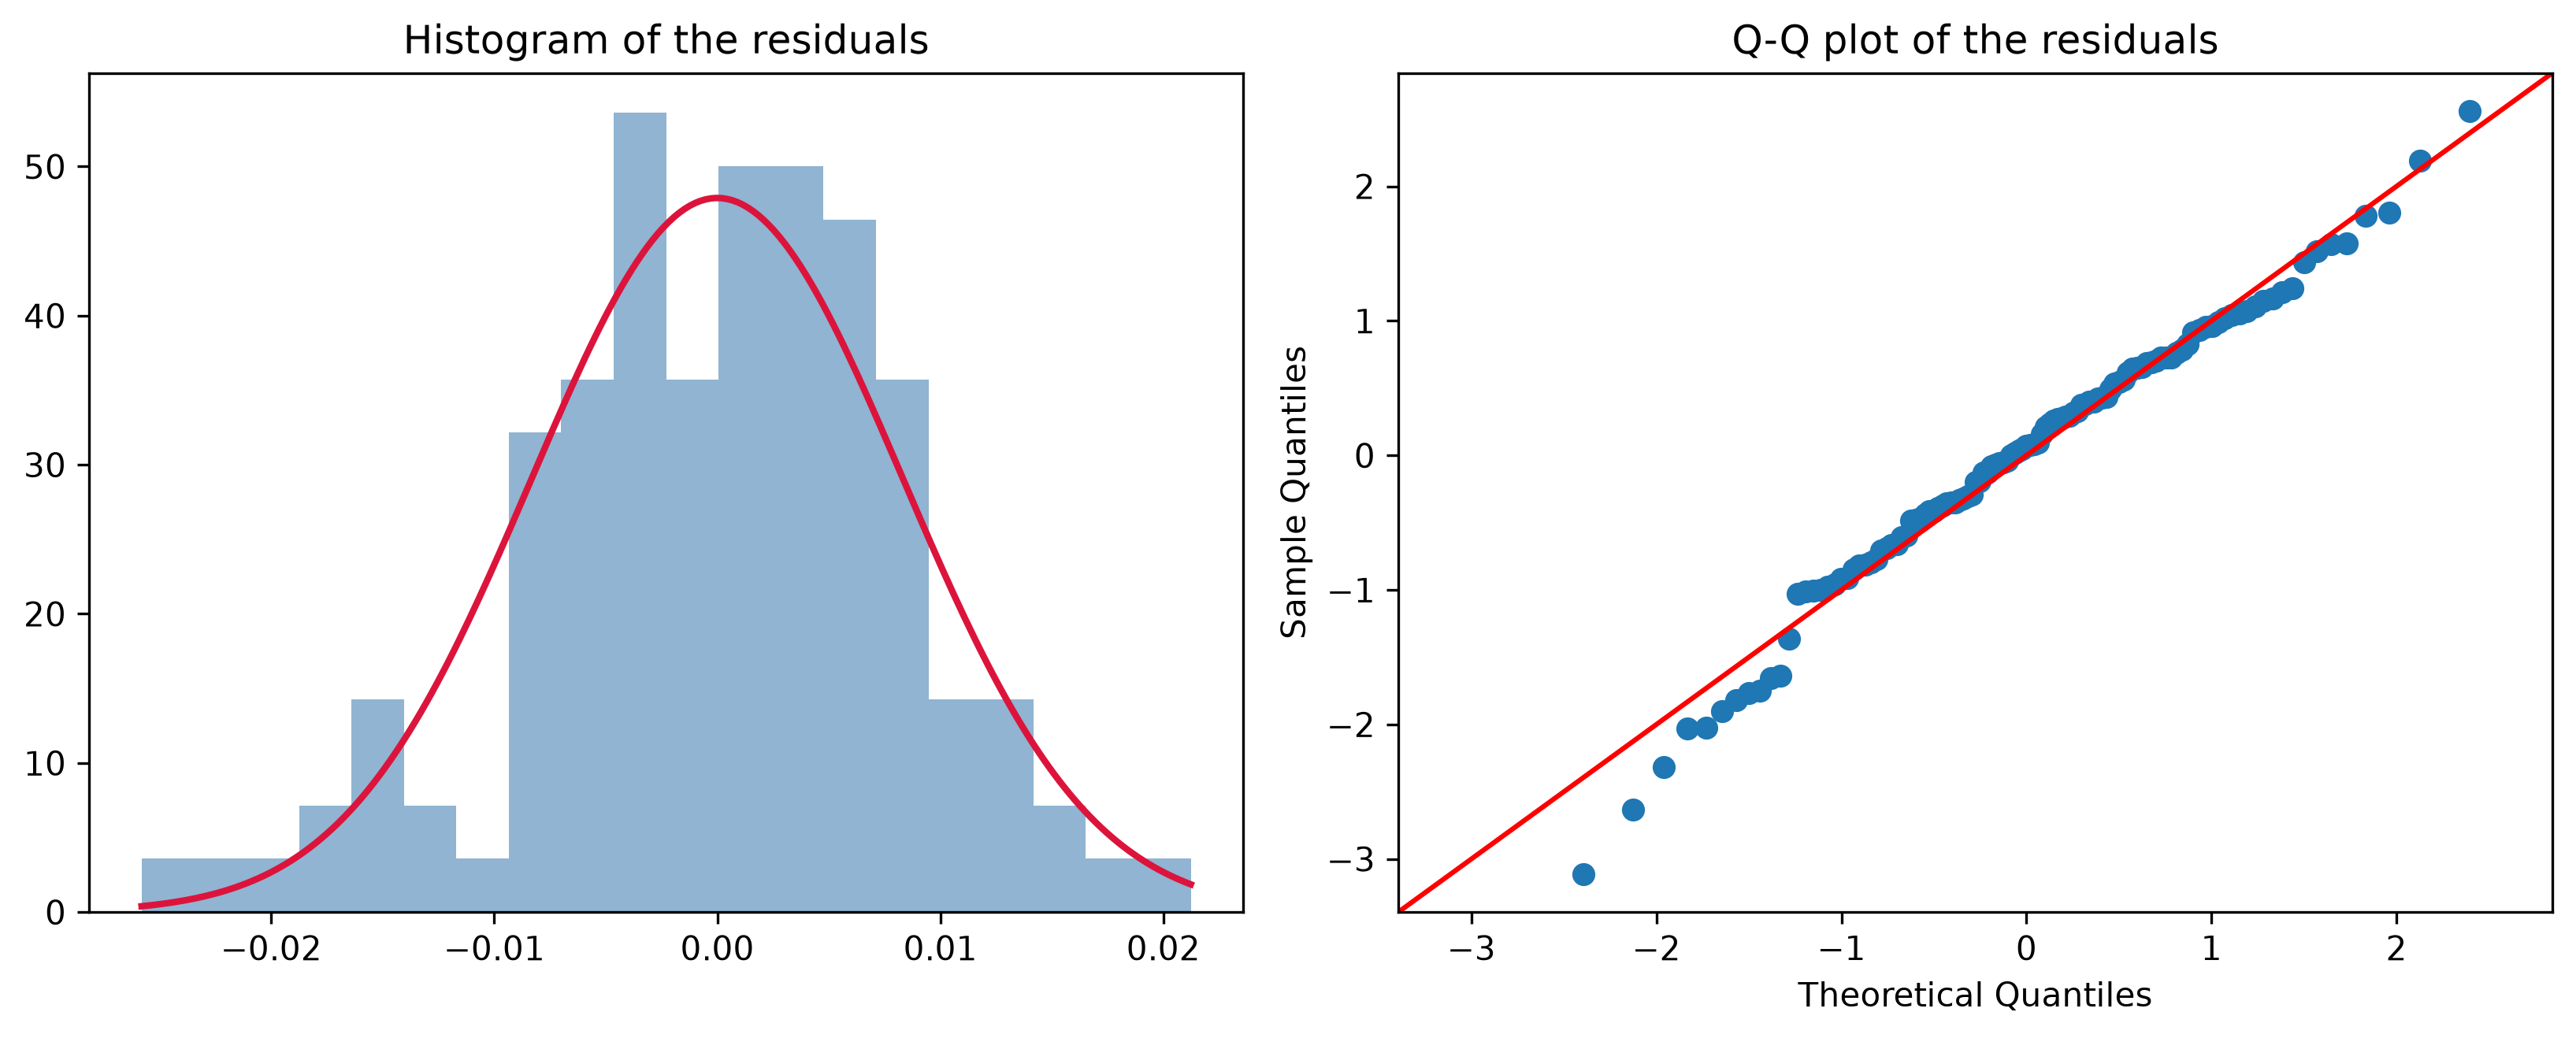
\includegraphics[width=\textwidth]{residuals_normality.png}
\caption{Histogram and Q-Q plot of the residuals of the bond model}
\label{fig:qq}
\end{figure}

\subsection{Influential observations}

Cook's distance measures how much the coefficients would change if an observation were removed. Six observations exceed the usual threshold $4/n = 0.0336$: December 2018, March 2020 and several months of 2022. They match well-known market episodes: the equity sell-off at the end of 2018, the COVID-19 crash and the rapid rate hikes of 2022. Most were already flagged by the IQR rule.

They are kept because they are real events and show how the fund behaves under stress. However, March 2020 stands out with a distance of 2.66, well above 1, so the estimates partly depend on this single month.

\begin{figure}[H]
\centering
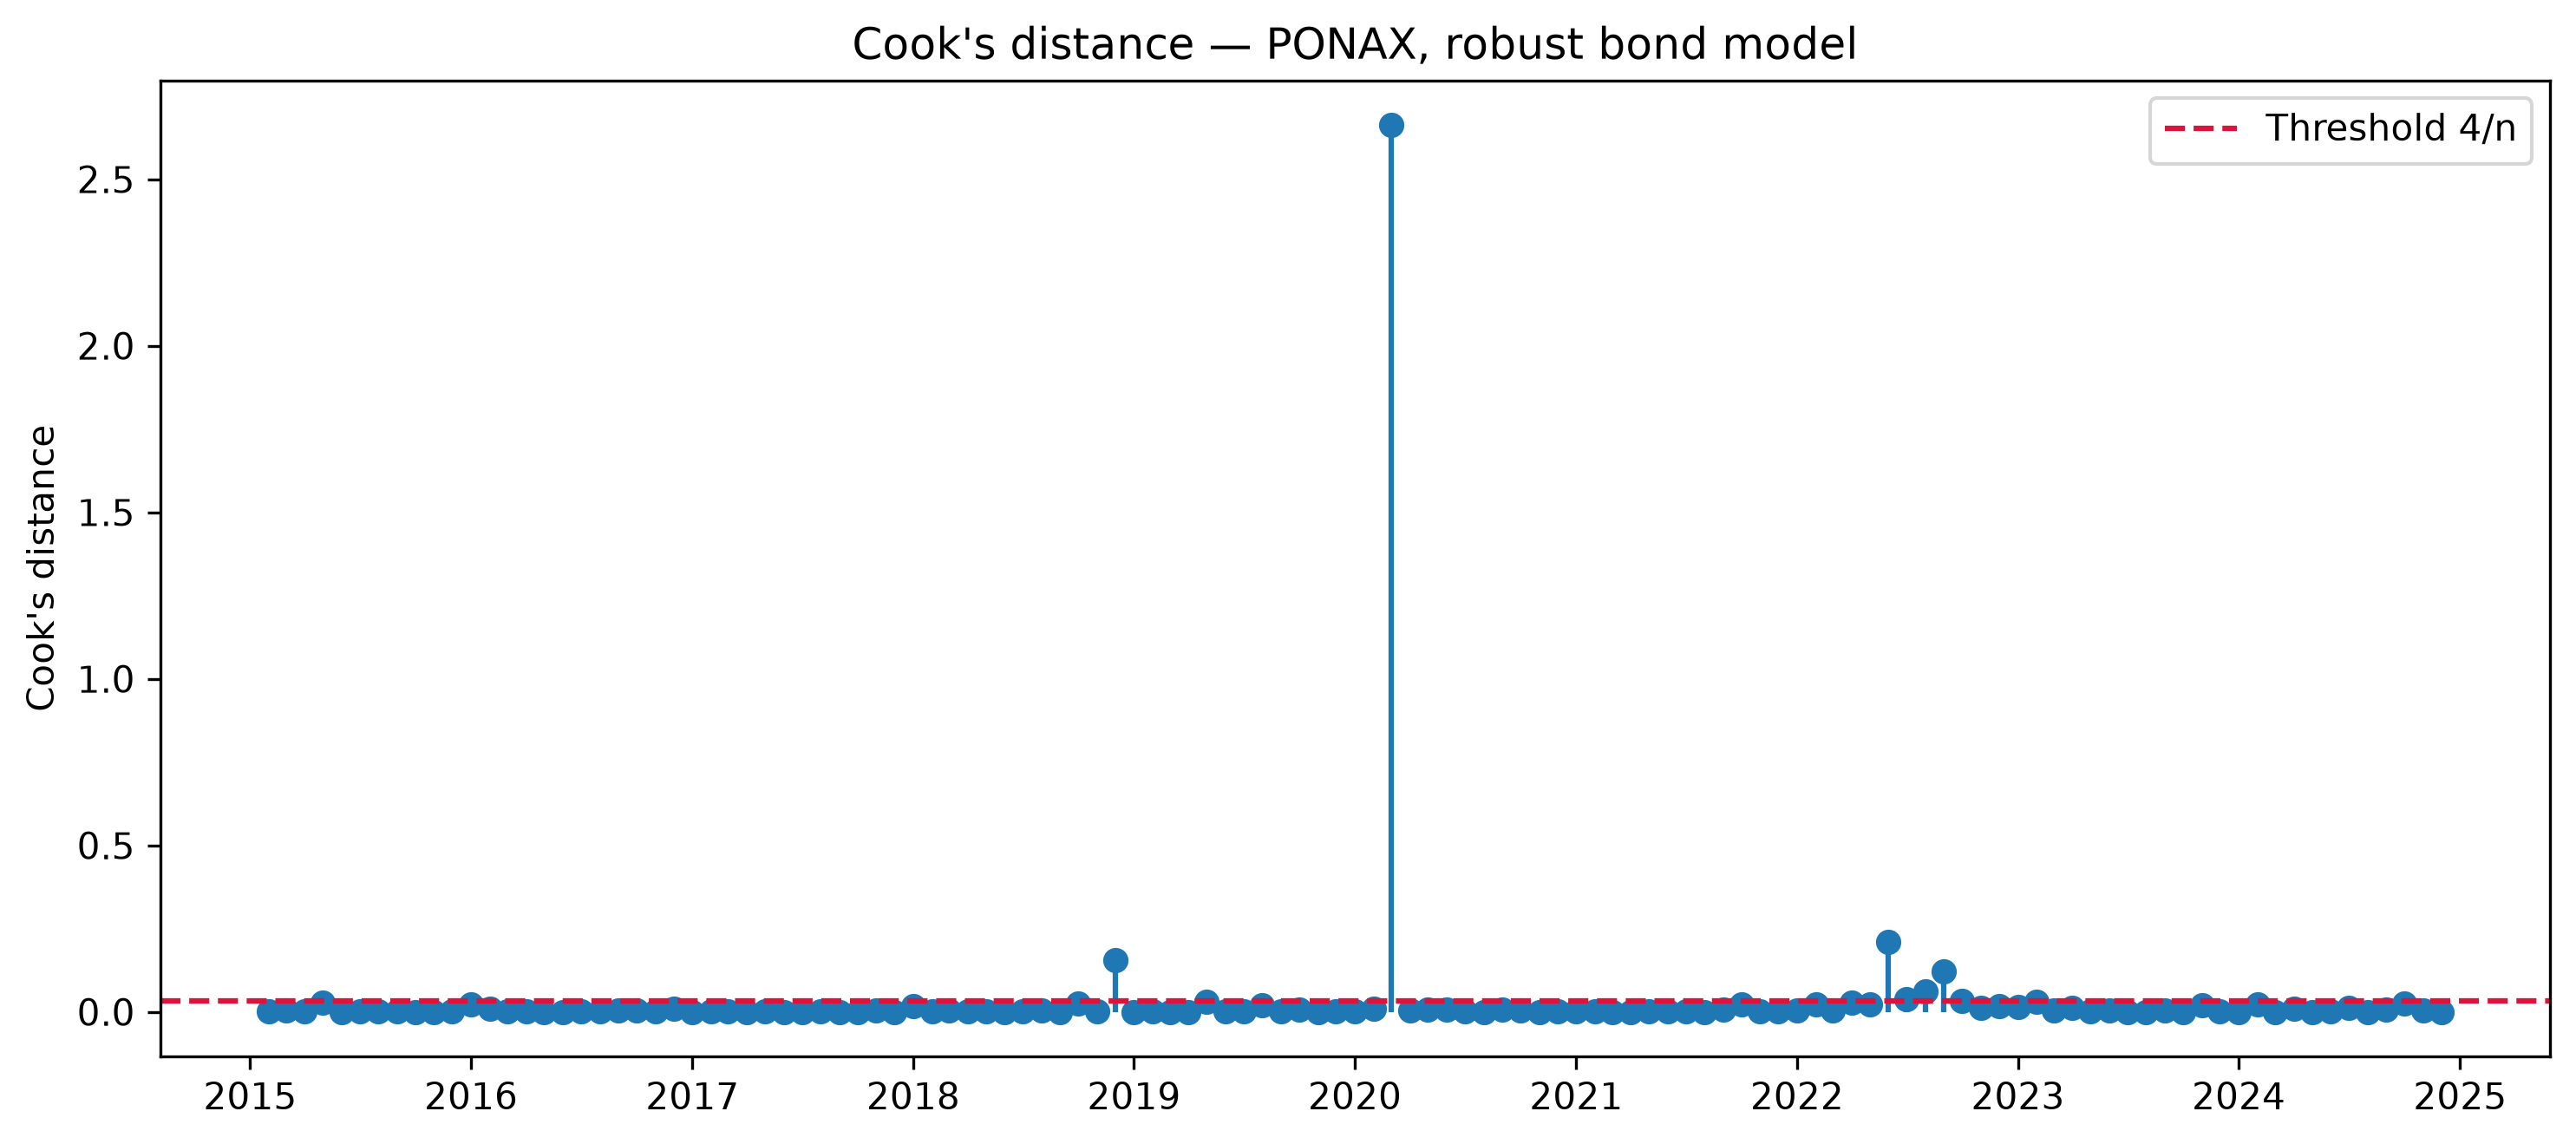
\includegraphics[width=0.8\textwidth]{cook_distance.png}
\caption{Cook's distance of the bond model (threshold $4/n$)}
\end{figure}

\subsection{Multicollinearity}

The variance inflation factor measures how much the variance of a coefficient is inflated by the correlation of its factor with the other regressors. All VIFs are below 1.2, far below the usual threshold of 5, which is consistent with the weak correlations observed in Section~3.

\subsection{Autocorrelation}

The Durbin--Watson statistic is 2.049, close to 2, so there is almost no first-order autocorrelation. The Breusch--Godfrey test up to order 6 gives a p-value of 0.065: the absence of autocorrelation is not rejected at the 5\% level, although the p-value is close to the threshold. Part~II returns to this point with a test at longer lags.

% =====================================================================
\part{Time-Series Modeling and Backtest}
% =====================================================================

\section{From the factor model to the time series}

The bond model explains about two thirds of PONAX's excess returns ($R^2 = 0.678$). The remaining third is in the residuals, and a well-specified model should leave nothing predictable in them. We test this with the Ljung--Box test:
\begin{equation}
Q(m) = n(n+2) \sum_{k=1}^{m} \frac{\hat{\rho}_k^2}{n-k},
\end{equation}
where $n$ is the number of observations and $\hat{\rho}_k$ the autocorrelation of the residuals at lag $k$. Under $H_0$ (no autocorrelation up to lag $m$), $Q(m)$ follows a $\chi^2$ distribution with $m$ degrees of freedom.

\begin{table}[H]
\centering
\caption{Ljung--Box test on the residuals of the bond model}
\small
\begin{tabular}{ccc}
\toprule
Lags $m$ & $Q(m)$ & p-value \\
\midrule
12 & 32.99 & 0.0010 \\
\bottomrule
\end{tabular}
\end{table}

$H_0$ is rejected: the residuals are not white noise, so part of the dynamics of the fund's returns is not captured by the factors. Since the Breusch--Godfrey test up to lag 6 did not reject the absence of autocorrelation, this structure probably lies at longer lags.

This raises the second question of the study:
\begin{center}
\emph{Can PONAX's past returns forecast its excess return more accurately than the historical mean?}
\end{center}
To answer it, we model the fund's excess return $R^e_t$ directly with an ARMA model and evaluate its forecasts out of sample.

\section{Method}

\subsection{Train and test samples}

We keep one full year, 2024, as the test period, the same horizon as a conventional 80/20 split on five years of data. With almost ten years of data, this gives a 90/10 split. The test sample is never used for estimation, otherwise forecast performance would be overstated.

\begin{table}[H]
\centering
\caption{Train/test split}
\small
\begin{tabular}{lcccc}
\toprule
Sample & Start & End & Observations & Share \\
\midrule
Training & 02/2015 & 12/2023 & 107 & 90\% \\
Test & 01/2024 & 12/2024 & 12 & 10\% \\
\bottomrule
\end{tabular}
\end{table}

\subsection{Stationarity}

An ARMA model requires a stationary series. The augmented Dickey--Fuller test, with the number of lags chosen by the BIC, gives a statistic of $-10.03$ on the training sample, far below the 5\% critical value of $-2.89$ ($p < 0.0001$). The unit root hypothesis is rejected: the excess return series is stationary and can be modeled in levels.

\subsection{Model selection}

An ARMA$(p,q)$ model is written
\begin{equation}
R^e_t = c + \sum_{i=1}^{p} \phi_i R^e_{t-i} + \varepsilon_t + \sum_{j=1}^{q} \theta_j \varepsilon_{t-j},
\end{equation}
where $\varepsilon_t$ is white noise.

The correlograms give a first indication (Figure~\ref{fig:acf}). Apart from lag 9, which is most likely due to chance, the autocorrelations and partial autocorrelations of the training sample all stay within the 95\% confidence band: the series looks like white noise.

\begin{figure}[H]
\centering
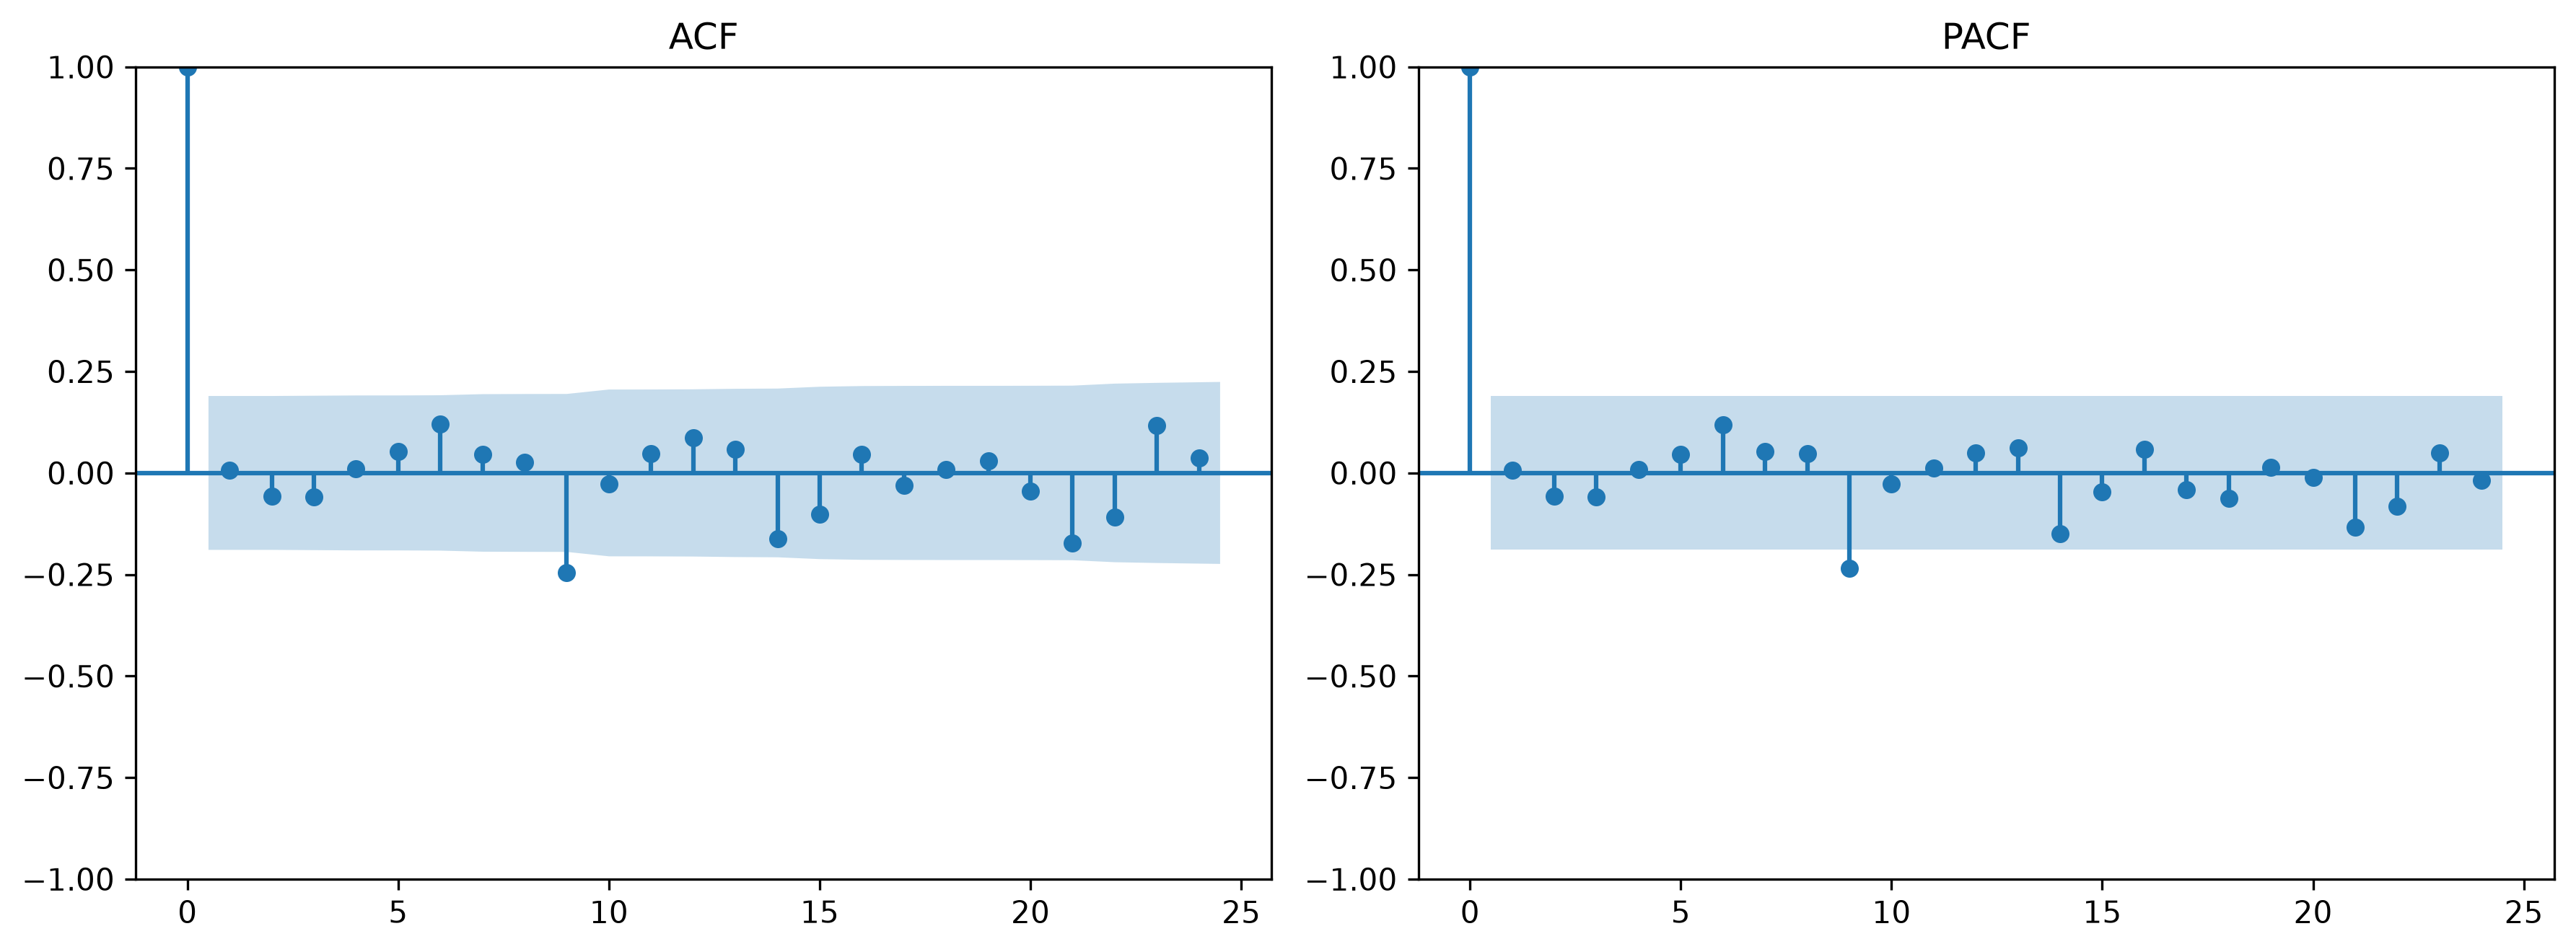
\includegraphics[width=\textwidth]{correlogram_ACF_PACF.png}
\caption{ACF and PACF of PONAX's excess return on the training sample}
\label{fig:acf}
\end{figure}

To choose the orders formally, we estimate all ARMA$(p,q)$ models with $p, q \in \{0, 1, 2, 3\}$ and compare their AIC and BIC.

\begin{table}[H]
\centering
\caption{Information criteria of the six best models}
\small
\begin{tabular}{ccrr}
\toprule
$p$ & $q$ & AIC & BIC \\
\midrule
0 & 0 & $-593.88$ & $-588.53$ \\
1 & 0 & $-591.88$ & $-583.86$ \\
0 & 1 & $-591.88$ & $-583.86$ \\
2 & 0 & $-590.25$ & $-579.56$ \\
0 & 2 & $-590.24$ & $-579.55$ \\
1 & 1 & $-589.65$ & $-578.96$ \\
\bottomrule
\end{tabular}
\end{table}

Both criteria select ARMA$(0,0)$, i.e.\ $R^e_t = c + \varepsilon_t$. The AR(1) and MA(1) models have an AIC about 2 points higher, which corresponds to the penalty for one extra parameter: adding the previous month's return or error barely improves the likelihood. The estimated constant is $\hat{c} = 0.0020$, or 0.20\% per month, but it is not significantly different from zero ($p = 0.252$).

\subsection{Diagnostics of the selected model}

The residuals of ARMA$(0,0)$ are simply the demeaned returns. They show no first-order autocorrelation (Ljung--Box at lag 1, $p = 0.95$). Their distribution is, however, far from normal: the Jarque--Bera statistic is 534.44 ($p < 0.001$), with a skewness of $-2.03$ and a kurtosis of 13.17. Their variance is also not constant: the heteroskedasticity test gives $H = 6.73$ ($p < 0.001$), meaning the variance is about 6.7 times higher at the end of the training sample (roughly 2021 to 2023) than at its start (2015 to 2017).

\section{Forecast and backtest}

\subsection{Forecast}

The model estimated on the training sample forecasts the twelve months of 2024. Since an ARMA$(0,0)$ has no memory, the forecast is the same for every month, $\hat{c} = 0.0020$, and so is the 95\% confidence interval $\hat{c} \pm 1.96\,\hat{\sigma}$, which ranges from about $-0.027$ to $0.031$. Uncertainty does not grow with the horizon.

\subsection{Out-of-sample evaluation}

\begin{figure}[H]
\centering
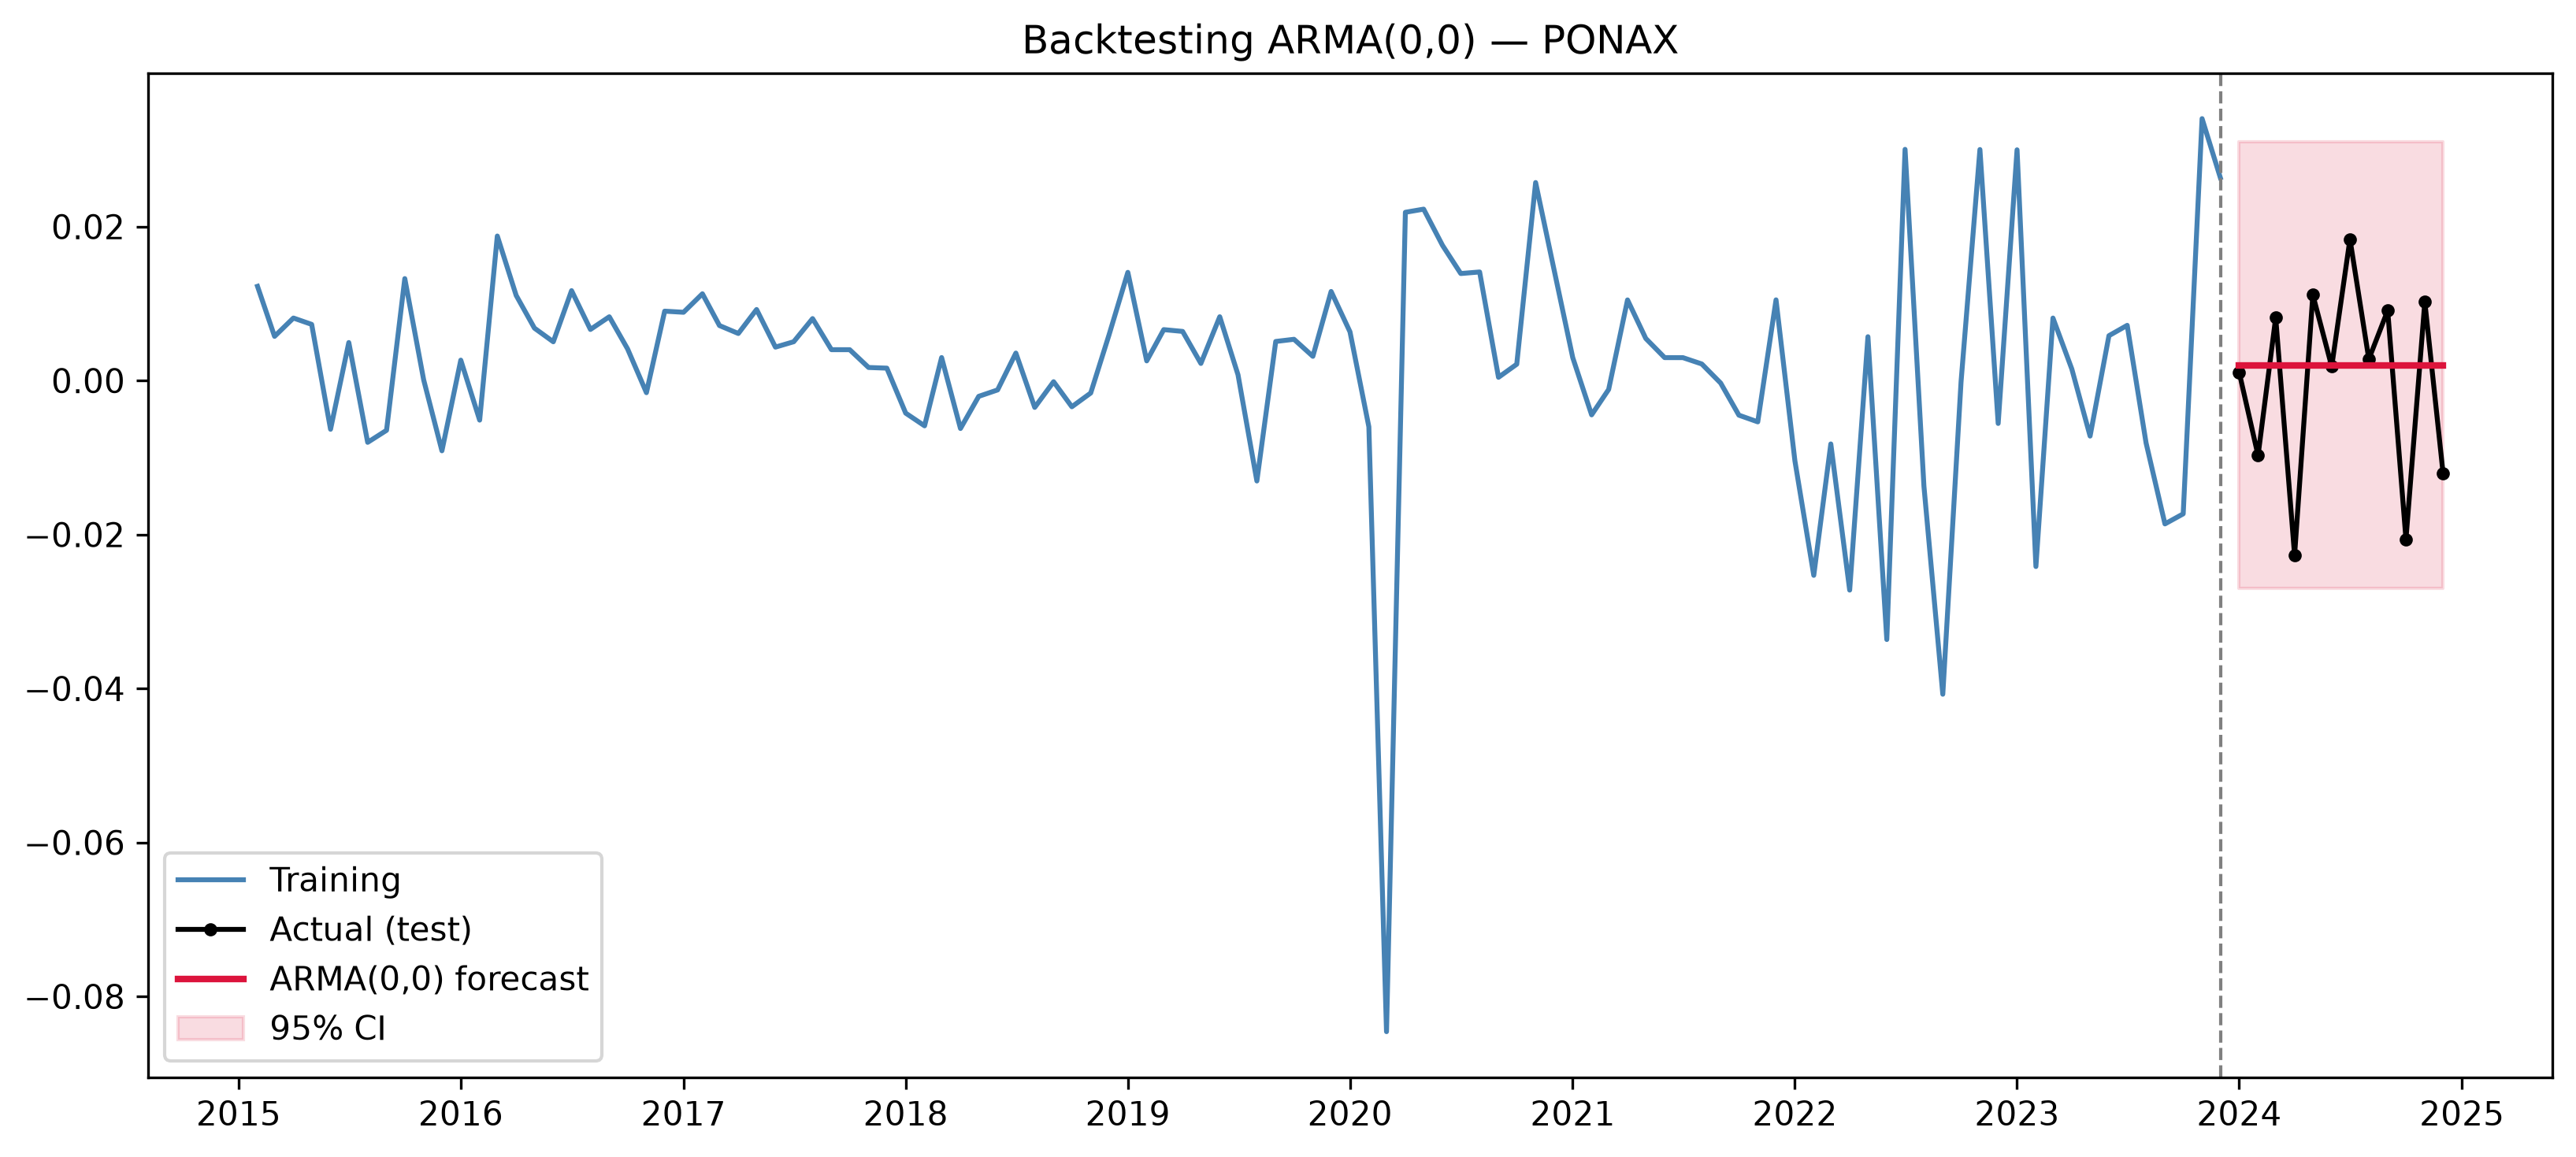
\includegraphics[width=\textwidth]{backtesting_ARMA(0,0).png}
\caption{Backtest of the ARMA$(0,0)$ model on 2024: training data, actual values, forecast and 95\% confidence interval}
\end{figure}

The returns observed in 2024 all fall within the confidence interval, but the flat forecast misses their month-to-month movements, which range from $-2.3\%$ to $+1.8\%$. We measure forecast accuracy over the $h = 12$ test months with
\begin{equation}
\text{RMSE} = \sqrt{\frac{1}{h}\sum_{t=1}^{h}\left(R^e_t - \hat{R}^e_t\right)^2},
\qquad
\text{MAE} = \frac{1}{h}\sum_{t=1}^{h}\left|R^e_t - \hat{R}^e_t\right|,
\end{equation}
and compare it with a naive forecast equal to the mean of the training sample.

\begin{table}[H]
\centering
\caption{Forecast errors on the 2024 test sample}
\small
\begin{tabular}{lcc}
\toprule
Model & RMSE & MAE \\
\midrule
ARMA$(0,0)$ & 0.0128 & 0.0102 \\
Naive forecast (historical mean) & 0.0128 & 0.0102 \\
\bottomrule
\end{tabular}
\end{table}

The two forecasts have identical errors. This is expected: the forecast of an ARMA$(0,0)$ is its estimated constant, which is virtually equal to the historical mean of the training sample. The best ARMA specification is the naive forecast itself.

\textbf{Answer to the second question:} PONAX's past returns do not improve the forecast of its future excess return. The residual autocorrelation found in the factor model cannot be exploited with an ARMA model of the fund's returns.

% =====================================================================
\section{Discussion}
% =====================================================================

\subsection{Interpretation}

The bond model explains about two thirds of the variability of PONAX's excess returns through three significant exposures: the equity market, interest rate risk and credit risk. Once these exposures are accounted for, the fund's alpha is not significant: its performance is in line with the risks it takes. The time-series analysis reaches a consistent conclusion from another angle: beyond its factor exposures, the fund's return history contains no structure that a simple ARMA model can use, and the ARMA specification selected by AIC and BIC reduces to the historical mean.

\subsection{Limitations}

\begin{itemize}
\item \textbf{Sample size.} 119 months is a short history. The test on the alpha has limited power, so a small outperformance cannot be ruled out. The backtest relies on only 12 test months and a single train/test split, which limits how general its conclusion is.
\item \textbf{Factor measurement.} TERM and DEF are built from monthly average rates, while fund returns are measured from month end to month end. DEF also uses Baa bonds, which are investment grade, whereas PONAX can hold up to 50\% in high yield, so it only partly captures the fund's credit exposure.
\item \textbf{Specification of the factor model.} The RESET test rejects linearity at the 5\% level, so the model could be better specified, and the estimates partly depend on March 2020, a highly influential observation.
\item \textbf{Assumptions of the ARMA model.} ARMA assumes a constant variance and normal errors. Both are rejected for PONAX's excess returns, so the forecast confidence interval is only approximate.
\end{itemize}

\subsection{Possible extensions}

\begin{itemize}
\item Build TERM and DEF from end-of-month rates, to align factors and returns in time.
\item Add a high yield credit factor, to better measure the fund's credit exposure.
\item Estimate the factor model on sub-periods, to check whether the results depend on March 2020 and on the 2022 rate hikes.
\item Model the time-varying volatility of returns (for example with a GARCH-type model), since the variance of the residuals is clearly not constant.
\item Evaluate forecasts on a rolling window rather than a single split, to obtain many more test points.
\end{itemize}

\section{Conclusion}

PONAX's Jensen's alpha is not significantly different from zero once its exposures to the equity market, interest rate risk and credit risk are taken into account, and its past returns do not forecast its future excess return better than the historical mean. Over 2015--2024, the fund's performance is explained by the risks it takes, not by abnormal or predictable returns.

\end{document}
